
%(BEGIN_QUESTION)
% Copyright 2005, Tony R. Kuphaldt, released under the Creative Commons Attribution License (v 1.0)
% This means you may do almost anything with this work of mine, so long as you give me proper credit

{\it Time-delay relays} are important circuit elements in many applications.  Determine what each of the lamps will do in the following circuit when pushbutton ``A'' is pressed for 10 seconds and then released:

$$\includegraphics[width=15.5cm]{i02500x01.eps}$$

Show your answer by completing this timing diagram:

$$\includegraphics[width=15.5cm]{i02500x02.eps}$$

For each of the relay contacts shown in this circuit, identify whether it would be properly called an {\it on-delay} or an {\it off-delay} contact.

\underbar{file i02500}
%(END_QUESTION)





%(BEGIN_ANSWER)

$$\includegraphics[width=15.5cm]{i02500x03.eps}$$

Each contact with an arrowhead pointed {\it toward} the energized position is an {\bf on-delay} contact, whereas each contact with an arrowhead pointed {\it away} from the energized position (i.e. toward the ``normal'' state) is an {\bf off-delay} contact.

\vskip 10pt

Time-delay relays are not the easiest for some students to understand.  The purpose of this question is to introduce students to the four basic types of time-delay relay contacts and their respective behaviors.  Discuss with your students how the contact symbols make sense (arrows on the switch actuators describing direction of delay).

Note to your students how it is possible to have different types of time-delay contacts actuated by the same relay coil.

%(END_ANSWER)





%(BEGIN_NOTES)


%INDEX% Electronics review: time-delay relay

%(END_NOTES)


